\documentclass[a4paper, 11pt]{article}

\usepackage[T1]{fontenc}
\usepackage[utf8]{inputenc}
\usepackage[english, italian]{babel}
\usepackage{biblatex}
\usepackage{amsmath}
\usepackage{hyperref}
\usepackage{graphicx}
\usepackage{listings}
\usepackage{tabularx}
\usepackage{booktabs,caption}
\usepackage[flushleft]{threeparttable}

\addbibresource{Bibliografia.bib}

\newcommand{\R}{\raggedleft\arraybackslash}

\author{Marco Mantovani}
\title{WarpSort}

\begin{document}
	\maketitle
	\begin{abstract}
		L'obiettivo di questo progetto per l'esame di \emph{GPU Computing} è la realizzazione dell'algoritmo di ordinamento \emph{WarpSort}
		presentato nell'articolo \cite{main} su scheda GPU Nvidia con il linguaggio \emph{CUDA C}.
	\end{abstract}
	\section{Introduzione}
		Il progetto si basa sui contenuti dell'articolo \cite{main} in cui viene descritto 
		l'algoritmo \emph{WarpSort} per l'ordinamento di vettori
		di grandi dimensioni su GP-GPU Nvidia.
		Il progetto è stato svolto su una scheda Nvidia GeForce 940MX \cite{GeForce}
		con capability 5.0. Ovviamente questa scheda non
		è la migliore per questo tipo di algoritmi (essendo una Maxwell è dedicata al settore videogame e non al campo computing). 
		
		Questo algoritmo sfrutta fortemente il concetto di \emph{warp} introdotto da Nvidia per le sue GPU.
		Un warp è un gruppo di 32 thread che lavora in SIMT (Single Instruction Multiple Threads), ovvero una configurazione
		dove la stessa istruzione viene eseguita dai 32 thread del warp su dati diversi ma in cui è anche consentito che i thread prendano
		percorsi diversi (in questo caso si parla di divergenza). 
		Se i thread di un warp divergono, il warp esegue serialmente ogni branch path,  disabilitando i thread che non appartengono a quel dato 
		path. Questo ovviamente porta ad un degrado delle performance. Nel momento in cui i branch path convergono i thread del warp 
		riprendono ad eseguire parallelamente. Esiste quindi una sincronizzazione implicita dei thread di un warp. Proprio su questa 
		sincronizzazione fa forza l'algoritmo WarpSort (che non a caso prende questo nome).
		Infatti questa sincronizzazione è legata alla struttura hardware della scheda e quindi è molto meno costosa di una sincronizzazione 
		esplicita.
	
	\section{Algoritmo}
		L'algoritmo si divide in 4 fasi principali più una fase preliminare. 
		Di queste cinque fasi, la terza è interamente svolta dalla CPU, che ha mostrato migliori performance della GPU.
		Le fasi 1, 2, 3 e 4 vanno eseguite in sequenza, ma la fase 0 può essere eseguita concorrentemente alle fasi 1 e 2 come mostrato
		nella figura \ref{fig:activitydiagram}.
		Nella figura \ref{fig:fasiprincipali} invece viene mostrato come le 4 fasi principali lavorano sull'array da ordinare.
		
		\begin{figure}
			\centering
			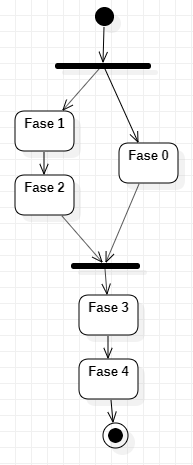
\includegraphics[width=0.3\linewidth]{img/ActivityDiagram}
			\caption{Activity Diagram del WarpSort}
			\label{fig:activitydiagram}
		\end{figure}		
		\begin{figure}
			\centering
			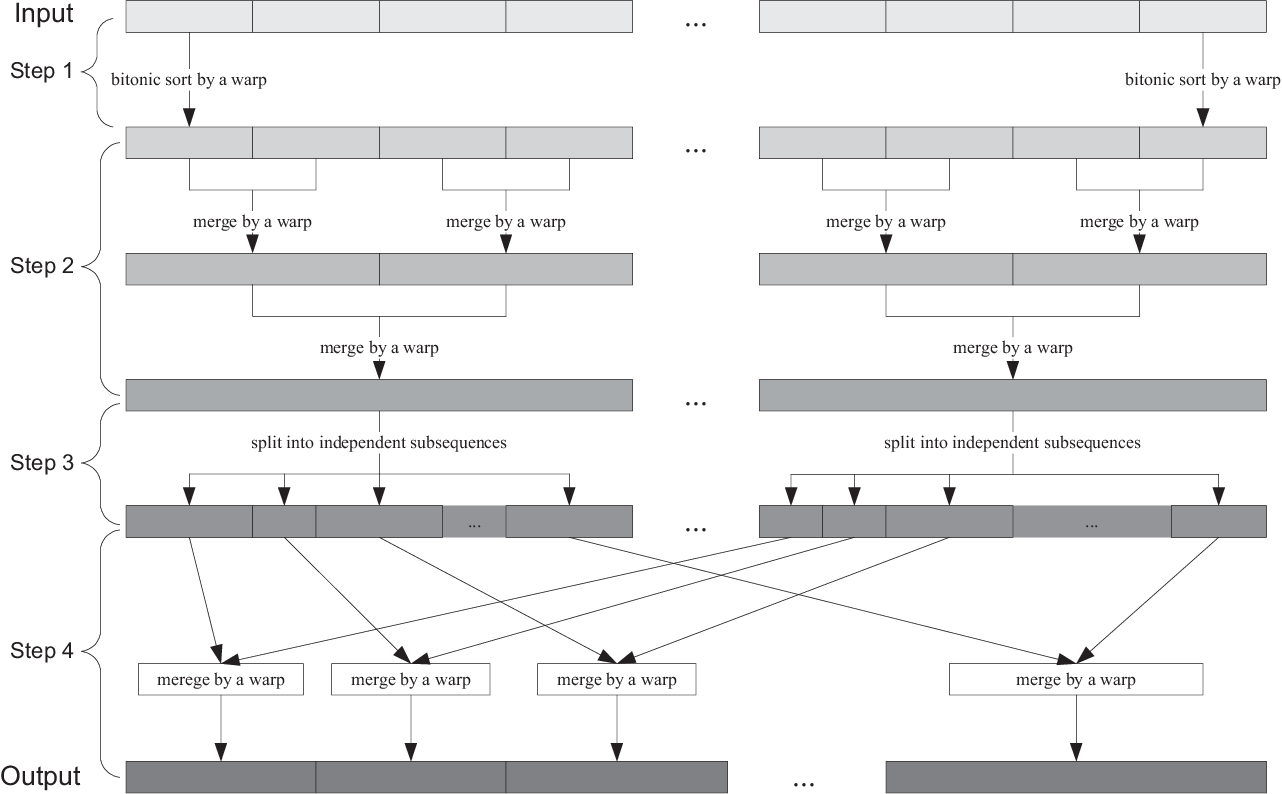
\includegraphics[width=0.9\linewidth]{img/fasiPrincipali}
			\caption{Il lavoro delle 4 fasi principali sull'array}
			\label{fig:fasiprincipali}
		\end{figure}
		
		\subsection{Preparazione dell'input}
			\label{preInput}
			Questo algoritmo necessità che l'input sia di lunghezza  $N$, con $N$ multiplo di una potenza di $2$.
			A questo scopo viene calcolato il parametro 
			$$MULT = 2^{3 * (\lfloor \log_{10} N\rfloor + 1)}$$ 
			Viene quindi esteso l'array fino al raggiungimento della lunghezza $M$, dove $M$ è il più piccolo multiplo di $MULT$ maggiore
			o uguale a $N$.
			Durante l'estensione viene aggiunto in coda all'array il valore $\infty$ (INFINITY) che fa da padding.
		
		\subsection{Fase 0 - Preliminare}
			\label{fase0}
			La fase preliminare consiste delle seguenti sottofasi:
			\begin{enumerate}
				\item Campionare l'array iniziale (non ordinato) estraendo così un sotto-array che chiameremo \emph{sample} di dimensioni $K*S$ 
				(operazione eseguita dalla CPU);
				\item Ordinare \emph{sample} (operazione eseguita dalla GPU);
				\item Estrarre da \emph{sample} tutti gli elementi che si trovano a distanza $K$ partendo dal primo, creando così
					un array ordinato di dimensione $S$ che chiameremo \emph{splitters} (operazione eseguita dalla CPU).
			\end{enumerate} 
			L'array \emph{splitters} servirà poi per sviluppare la fase 3.
			
			La fase 0 è caratterizzata da due valori: $S$ e $K$.
			È fondamentale che $K$ e $S$ siano potenze di $2$, tali che $S*K \geq 128$.
			Il valore $K$ è stato definito come costante, 
			mentre il valore $S$ è dato dalla seguente formula			
			$$S = C * 2^{\lceil \log_2 \lfloor \log_{10} N \rfloor + 1 \rceil}$$
			dove $N$ è la dimensione dell'array da ordinare e 
			$C$ è una costante (sempre potenza di $2$). 
			Dopo diverse prove è sembrata una buona scelta porre $K = 32$ e $C = 64$.
			
			Per eseguire la sottofase 2 si è seguita la seguente procedura:
			\begin{enumerate}
				\item Dividere \emph{sample} in gruppi di $128$ elementi;
				\item Eseguire \emph{bitonic\_sort} \cite{BS} (vedi fase 1 alla sottosezione \ref{fase1});
				\item Unire i gruppi di 128 a due a due attraverso \emph{bitonic\_merge} \cite{BS} (vedi fase 2 alla sottosezione \ref{fase2}) 
				fino ad riottenere un unico array.
			\end{enumerate}
		
			Proprio dalla divisione in gruppi da $128$ e poi dalla riunione a coppie nasce l'esigenza di avere $S*K$ potenza 
			di $2$, maggiore di $128$.
			
			La figura \ref{fig:fase0} mostra i procedimenti eseguiti nelle sottofasi della fase 0
			(senza illustrare i dettagli della sottofase 2).
			
			\begin{figure}
				\centering
				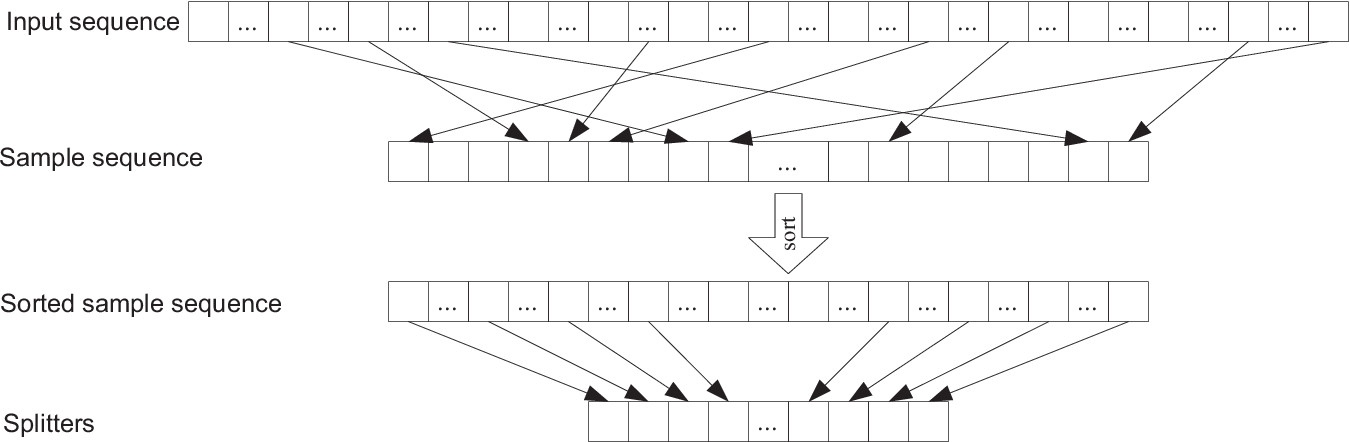
\includegraphics[width=0.9\linewidth]{img/fase0}
				\caption{Illustrazione delle sottofasi della fase 0}
				\label{fig:fase0}
			\end{figure}
			
		\subsection{Fase 1 - Bitonic Sort}
			\label{fase1}
			Questa fase suddivide l'array in gruppi da 128 elementi e usa la funzione \emph{bitonic\_sort} sulla GPU per
			ordinare i sotto-array.
			Il kernel viene lanciato con blocchi da 32 thread (ovvero da un warp).
			
			Questa fase viene eseguita in parallelo con la fase 0.
			
			Ogni blocco ordina un sotto-array da 128 elementi seguendo lo schema indicato nella figura 
			\ref{fig:bitonicsort}
			(notare che nella figura avviene un \emph{bitonic\_sort} con sotto-array di 16 elementi, ma l'estensione a 128 è immediata).
			
			Questo algoritmo del bitonic sort consiste di $\log_2(128) = 7$ fasi, dove la $k$-esima fase (con $0 \leq k \leq \log_2(128)$) è 
			composta da $k+1$ passi.
			In ogni fase vengono selezionate coppie di due elementi ed eseguite operazioni di confronto e scambio (con riferimento alla figura
			\ref{fig:bitonicsort} la freccia, dopo il confronto e il possibile scambio, deve puntare all'elemento maggiore). 
			Tra due passi adiacenti (e quindi anche tra due fasi adiacenti) è necessaria una sincronizzazione globale dei thread che lavorano 
			allo stesso	sotto-array. 
			Per evitare questo sovraccarico di sincronizzazione l'algoritmo ordina ogni sotto-array attraverso un warp, piuttosto 
			che per blocco. In questo modo si sfrutta il vantaggio dell'esecuzione sincrona di thread in un warp, 
			per eliminare la necessità di barriere esplicite.
			
			Come si può vedere nella figura \ref{fig:bitonicsort} tutte le fasi tranne l'ultima si basano sulla stessa rete di comparatori, 
			mentre l'ultima fase, che varia rispetto alle precedenti, è detta \emph{bitonic\_merge}.
			\begin{figure}
				\centering
				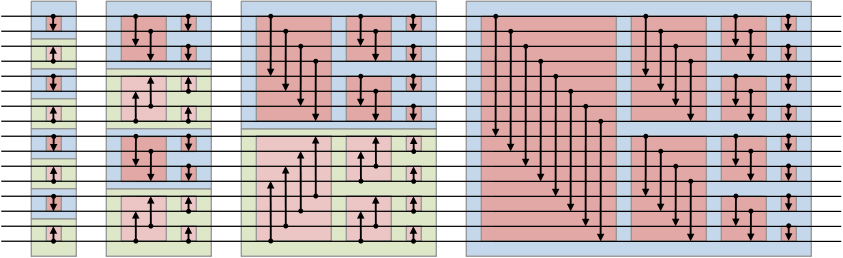
\includegraphics[width=0.9\linewidth]{img/BitonicSort}
				\caption{Bitonic\_sort di 16 elementi}
				\label{fig:bitonicsort}
			\end{figure}			
		\subsection{Fase 2 - Bitonic Merge}
			\label{fase2}
			Questa fase usa la funzione \emph{bitonic\_merge} sulla GPU (evidenziata nell'ultima fase della figura \ref{fig:bitonicsort}) per 
			fondere a due a due	i sotto-array creati nella fase precedente.			
			Il kernel viene lanciato con blocchi da 32 thread (ovvero da un warp).
			
			Questa fase non può iniziare fino a quando la fase 1 non è stata completata, ma procede in parallelo alla fase 0.
						
			Virtualmente questa fase divide l'array in una matrice di $l$ righe, dove ogni riga ha $n$ elementi ed è localmente ordinata.
			Inizialmente $n=128$ (questo grazie alla fase 1). 
			Le righe sono numerate da $0$ a $l-1$.
			L'algoritmo fonde parallelamente la riga $i$ con la riga $i+1$, con $i$ pari e compresa tra  $0$ e $l-2$ . 
			In questo modo $l$ si dimezza e $n$ si raddoppia ad ogni passo. 
			Per avere il massimo parallelismo e per permettere un corretto funzionamento della fase 4,
			l'algoritmo continua a fondere le righe fino a quando si verificano \emph{entrambe} le seguenti condizioni:
			\begin{enumerate}
				\item ci sono almeno $L$ righe ($L$ è una costante che dovrebbe essere maggiore del numero di SM della GPU. Per la mia GPU ho 
				scelto il valore $4$);
				\item $l$ è pari.
			\end{enumerate} 
			Il punto 1 garantisce che la fase 2 abbia una certo grado di parallelismo, mentre il punto 2 è importante per l'esecuzione della fase 
			4, dove viene richiesto che ogni riga abbia la stessa grandezza $n$.
		\subsection{Fase 3 - Splitting}
			\label{fase3}
			Questa fase ha il compito di dividere le $l$ righe di $n$ elementi generati alla fase precedente in $S + 1$ sotto-array, usando 
			i valori di	\emph{splitters} come punto di divisione.
			Questa fase avviene interamente su CPU in quanto, per questo lavoro, si è dimostrata molto più veloce della GPU.
			
			Questa fase non può iniziare fino a quando la fase 2 e la fase 0 non sono state completate.
			
			Questa fase semplicemente scorre l'array prodotto della fase 2 (che è virtualmente diviso in $l$ righe da $n$ elementi l'una) 
			riga per riga e, per ognuna, conta quanti elementi ci sono tra due valori consecutivi di \emph{splitters} 
			(che sono stati ordinati dalla fase 0). Questi contatori vengono salvati in una matrice $l \times (S+1)$ chiamata $local\_count$.
			
			Alla fine di questa fase si raggiunge (virtualmente) la configurazione rappresentata nella figura \ref{fig:fase3}.
			
			\begin{figure}
				\centering
				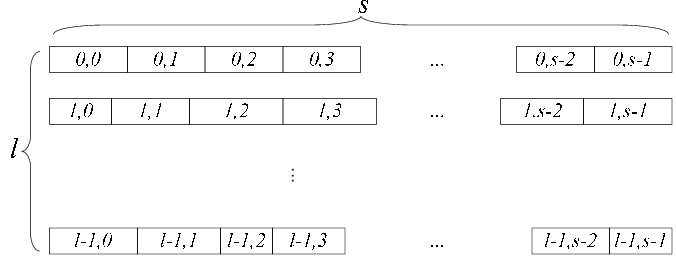
\includegraphics[width=0.7\linewidth]{img/fase3}
				\caption{Configurazione virtuale dell'array alla fine della fase 3}
				\label{fig:fase3}
			\end{figure}
			
		\subsection{Fase 4 - Final merge}
			\label{fase4}
			Questa fase ha il compito di unire i sotto-array generati dalla fase precedente al fine di generare l'array ordinato finale.
			Questa fase avviene su GPU attraverso la funzione \emph{bitonic\_merge\_2}.
			Il kernel viene lanciato con blocchi da 32 thread (ovvero da un warp).
			
			Questa fase non può iniziare fino a quando la fase 3 non è stata completata.
			
			Questa fase unisce i $k$-esimi sotto-array di ogni riga. Questi sotto-array sono localmente ordinati e  
			sono inclusi in un range comandato dai valori $k-1$ e $k$ di \emph{splitters}.
			Come illustrato nella figura \ref{fig:fasiprincipali}, questa fase porta a compimento l'ordinamento.
			
			Per svolgere questa fase si uniscono attraverso un \emph{bitonic\_merge} le righe $i$ e $i+1$ (con $i$ inizializzato a $0$). 
			Questo \emph{bitonic\_merge}, implementato dalla funzione \emph{bitonic\_merge\_2}, è però leggermente diverso da quello della fase 2.
			Infatti nella fase 2 c'è la certezza che i sotto-array sono di dimensione uguale e multipla di una potenza di $2$.
			In questa fase, invece, questa certezza non c'è, quindi la funzione deve occuparsi di mettere del padding 
			(come visto nella sottosezione \ref{preInput} si è usato il valore $\infty$)
			ai singoli sotto-array. 
			Questo padding porta le relative dimensioni al più vicino multiplo di $64$.
			I due sotto-array possono ancora avere dimensioni diverse, ma questo non causa problemi all'algoritmo.
			
			Quando $i$ supera il valore $l-1$ allora vuol dire che sono state unite tutte le righe e quindi che si è
			generato l'array ordinato finale.
	\section{Strategie}
		\label{strategie}
		Il codice prodotto cerca di sfruttare al massimo le potenzialità della GPU.
		In totale i kernel sono 3:
		\begin{enumerate}
			\item \emph{bitonic\_sort} usato dalla fase 0 e dalla fase 1
			\item \emph{bitonic\_merge} usato dalla fase 0 e dalla fase 2
			\item \emph{bitonic\_merge\_2} usato dalla fase 4
		\end{enumerate}
		
		\subsection{Warp divergence}
			I tre kernel non presentano warp divergence. 
			Questo è dovuto soprattutto alle ottimizzazioni introdotte dal compilatore, in quanto
			il codice deve obbligatoriamente presentare dei branch durante il confronto di due elementi 
			(confronto che poi può portare allo swap dei due).
		
		\subsection{Memorie}
			In tutti e tre i kernel si sono fatti accessi coalesced alla \emph{global memory}.
			Nei kernel 1 e 2 gli accessi sono stati anche allineati, per garantire il massimo delle performance. Nel kernel 4 
			invece l'allineamento non è stato possibile per via del problema, già evidenziato nella sottosezione \ref{fase4}, 
			legato alle dimensioni diverse dei sotto-array e alla necessità di aggiungere padding.
			
			Tutti e tre i kernel fanno uso della \emph{shared memory} in cui viene copiato integralmente o parzialmente 
			il/i sotto-array su cui il warp sta lavorando. Questo perché la rete generata dal bitonic\_sort fa accessi multipli 
			alle stesse locazioni, e quindi copiare questi dati dalla global alla shared memory ha aiutato le performance.
			Le copie dalla global memory alla shared memory (e viceversa) sono state progettate per garantire l'accesso coalesced e, tranne nel
			terzo kernel, allineato alla global memory. 
			
			Purtroppo i tre kernel non riescono ad evitare di causare dei \emph{bank conflict} durante l'accesso alla shared memory. 
			Questo è intrinsecamente legato al modo in cui avvengono gli accessi in memoria nella rete generata dal bitonic\_sort.
			Nonostante questo problema, l'uso della shared memory è comunque notevolmente più performante dell'uso della sola global memory 
			(che per di più senza la shared memory perderebbe l'accesso allineato e coalesced).  
		
			Infine si è optato per l'uso della memoria globale "classica" (ad uso esclusivo della GPU) in quanto ha dimostrato performace
			nettamente migliori della \emph{unified memory}.
			
			La \emph{pinned memory} è stata usata temporaneamente per permettere alla CPU di riempire l'array da ordinare. 
			In questo modo è stato possibile per lo stream della GPU copiarla in modo asincrono nella memoria device.
		\subsection{Unrolling}
			Nei kernel 1 e 3 si è usato l'unrolling per eliminare la presenza di tutti i cicli in cui il numero di iterazioni è conosciuto a
			compile-time. 
			Questo permette di velocizzare l'esecuzione del codice. 
			
		\subsection{Stream}
			Per sfruttare al massimo il parallelismo offerto dalla GPU sono stati creati due stream: 
			uno per la fase 0 e uno per le altre 4 fasi.			
			In particolare questo ha permesso l'esecuzione parallela della fase 0 con le fasi 1 e 2.
			
			Tutte le copie di memoria sono state rese asincronie tra CPU e stream. In questo modo la CPU ha modo di continuare la 
			computazione senza dover attendere che la copia in memoria sia terminata.			
			
		\subsection{Event}
			Per calcolare il tempo impiegato dall'intero algoritmo di ordinamento si è sfruttato lo stream di default (o stream 0)
			in cui sono stati inseriti due eventi: uno prima di iniziare l'ordinamento e il secondo alla fine dell'ordinamento.
			La differenza tra i timestamp di questi due eventi ha permesso una misurazione accurata del tempo impiegato del warpsort per ordinare.
	\section{API}
		Per generare rapidamente i numeri random con cui popolare l'array da ordinare si è usata la libreria cuRAND. In questo modo è stata
		velocizzata notevolmente la generazione dei valori. 
	\section{Applicazione}
		L'applicazione richiede in input da linea di comando. Qui la specifica: 
		\begin{verbatim}
			{-f "path"| -t N | -i N | -r N} [-g] [-p S] [-c] [-o "path" | -s]
		\end{verbatim}
		dove:
		\begin{itemize}
			\item \emph{-f path} indica che l'array da ordinare è dal file \emph{path};
			\item \emph{-t $N$} indica che l'array da ordinare deve essere di dimensione $N$ (con $N > 0$) e deve essere generato randomicamente;
			\item \emph{-i $N$} indica che l'array da ordinare deve essere di dimensione $N$ (con $N > 0$) e deve essere letto da standard input;
			\item \emph{-r $N$} indica che l'array da ordinare deve essere di dimensione $N$ (con $N > 0$) e deve essere generato randomicamente
			 	(i numeri generati verranno stampati su standard output);
			\item \emph{-g} indica che si vogliono effettuare i controlli sull'ordine e sulla presenza di tutti e soli gli elementi dell'array 
			iniziale nell'array ordinato;
			\item \emph{-p S} indica che si vuole usare il seme $S$ per i generatori pseudo-randomici. Se questa opzione manca viene
				usata la funzione di sistema $time(NULL)$ per la generazione del seme;
			\item \emph{-c} indica che l'ordinamento deve essere decrescente. Se questa opzione manca l'ordinamento è crescente;
			\item \emph{-o path} indica che si vuole salvare l'array ordinato sul file \emph{path} (nel caso in cui il file esiste già, viene 
				sovrascritto);
			\item \emph{-s} indica che si vuole stampare l'array ordinato su standard output.
		\end{itemize}
	
		Finto l'ordinamento viene stampata su standard output una stringa così formata:
		\begin{verbatim}
			GPU warpsort ha ordinato <N> [<M>] elementi (<NG> [<MG>] GB) 
			in <S> secondi
		\end{verbatim}
		dove:
		\begin{itemize}
			\item $N$ è la grandezza dell'array;
			\item $M$ è la dimensione dell'array con il padding (per dettagli vedere la sottosezione \ref{preInput});
			\item $NG$ è la dimensione in GB di $N$;
			\item $MG$ è la dimensione in GB di $M$;
			\item $S$ è il tempo, espresso in secondi, impiegati per effettuare l'ordinamento (ovvero portare a termine le 5 fasi).
		\end{itemize}	
	\section{Profilazione}
		Per la profilazione si è usato il programma nvprof con il seguente comando:
		
		\begin{verbatim}
			nvprof --metrics branch_efficiency,gld_efficiency,
			                 gst_efficiency,sm_efficiency,shared_efficiency 
			       WarpSort_Mantovani.exe -t 134217728
		\end{verbatim}
		
		Nella tabella \ref{tab:prof} sono riportate le metriche medie per i tre kernel.
		\begin{table}[h]			
			\centering
			\begin{tabular}{c|ccc}
								    & bitonic\_sort & bitonic\_merge & bitonic\_merge\_2 \\
		        \hline
				branch\_efficiency  & 100.00\%      & 100.00\%       & 100.00\%          \\
				gld\_efficiency     & 100.00\%      & 100.00\%       &  77.27\%          \\
				gst\_efficiency     & 100.00\%      & 100.00\%       &  82.07\%          \\
				sm\_efficiency      &  95.42\%      &  95.62\%       &  99.28\%          \\
				shared\_efficiency  &  28.09\%      &  46.38\%       &  26.35\%          \\
				achieved\_occupancy &  47.54\%      &  31.97\%       &  46.90\%          \\
			\end{tabular}
			\caption{Tabella con le metriche di profilazione}
			\label{tab:prof}
			\end{table}
		
		Da questa tabella si può osservare, come già evidenziato nella sezione \ref{strategie}, che:
		\begin{itemize}
			\item la warp divergence è nulla per tutti e tre i kernel [vedi comando branch\_efficiency];
			\item per i primi due kernel l'accesso alla global memory è efficiente (quindi allineato e coalesced), 
				mentre nel terzo kernel è meno efficiente (infatti non è allineato) [vedi comandi gld\_efficiency e gst\_efficiency];
			\item l'uso degli SM è molto efficiente in tutti e tre i kernel [vedi comando sm\_efficiency];
			\item l'uso della shared memory provoca molti bank conflict, causando un cattivo uso della stessa [vedi comando shared\_efficiency];
			\item la quantità di warp attivi rispetto al numero massimo di warp per MS è medio/basso [vedi comando achieved\_occupancy].
		\end{itemize}
		
		Infine con lo strumento nvvp si è profilata l'esecuzione dei kernel nel tempo (timeline). Il risultato è nella figura \ref{fig:nvvp}.
		
		\begin{figure}
			\centering
			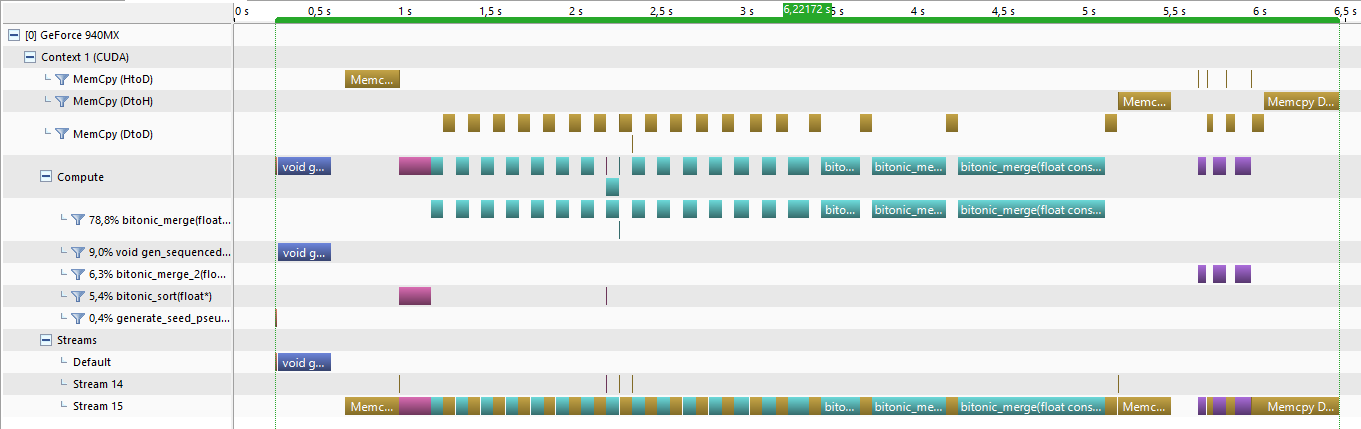
\includegraphics[width=0.99\linewidth]{img/nvvp}
			\caption{Profilazione NVVP}
			\label{fig:nvvp}
		\end{figure}
		
	\section{Test}
		Sono stati eseguiti diversi test sul warpsort. 
		In particolare, per avere un confronto con un ordinamento della CPU, si è scelto di realizzare un quick sort iterativo e di
		mettere a confronto i tempi.  
		Nella tabella \ref{tab:time} vengono riportati i tempi con diverse dimensioni dell'array iniziale.
		\begin{table}[h]			
			\centering
			\begin{tabularx}{\textwidth}
				{>{\R}X|>{\R}X|>{\R}X|>{\R}X}
				N° elementi [MB] & N° elementi + padding [MB] & Tempo CPU (millisecondi) & Tempo GPU (millisecondi)\\
				\hline
				  $10^1$   [0.00] & $2^{12}$   [0.02] &     0.04 &    2.18 \\			
				  $10^2$   [0.00] & $2^{13}$   [0.03] &     0.04 &    3.11 \\			
				  $10^3$   [0.00] & $2^{13}$   [0.03] &     0.09 &    2.82 \\				
				$2^{13}$   [0.03] &        =          &     0.53 &    2.28 \\
				  $10^4$   [0.04] & $2^{15}$   [0.13] &     0.67 &    4.63 \\
				$2^{15}$   [0.13] &        =          &     2.33 &    4.00 \\
				  $10^5$   [0.38] & $2^{18}$   [1.00] &     9.41 &   23.63 \\
				$2^{18}$   [1.00] &        =          &    19.17 &   14.31 \\
				  $10^6$   [3.81] & $2^{21}$   [8.00] &    78.80 &  146.12 \\
				$2^{21}$   [8.00] &        =          &   171.15 &   87.04 \\
				  $10^7$  [38.15] & $2^{24}$  [64.00] &   909.06 &  976.30 \\
				$2^{24}$  [64.00] &        =          &  1560.77 &  689.21 \\
				  $10^8$ [381.47] & $2^{27}$ [512.00] & 10088.44 & 6941.27 \\
				$2^{27}$ [512.00] &        =          & 13516.47 & 5871.02 \\
			\end{tabularx}
			\caption{Tabella con il confronto tra i tempi di GPU e CPU}
			\label{tab:time}
			\begin{tablenotes}
				\small
				\item \textbf{NOTA}: la GPU ordina sempre l'array con padding, mentre la CPU quello senza padding!
			\end{tablenotes}
		\end{table}
		
		Nella figura \ref{fig:confrontotempi} si può vedere un grafico che confronta i tempi ottenuti.
		
		\begin{figure}
			\centering
			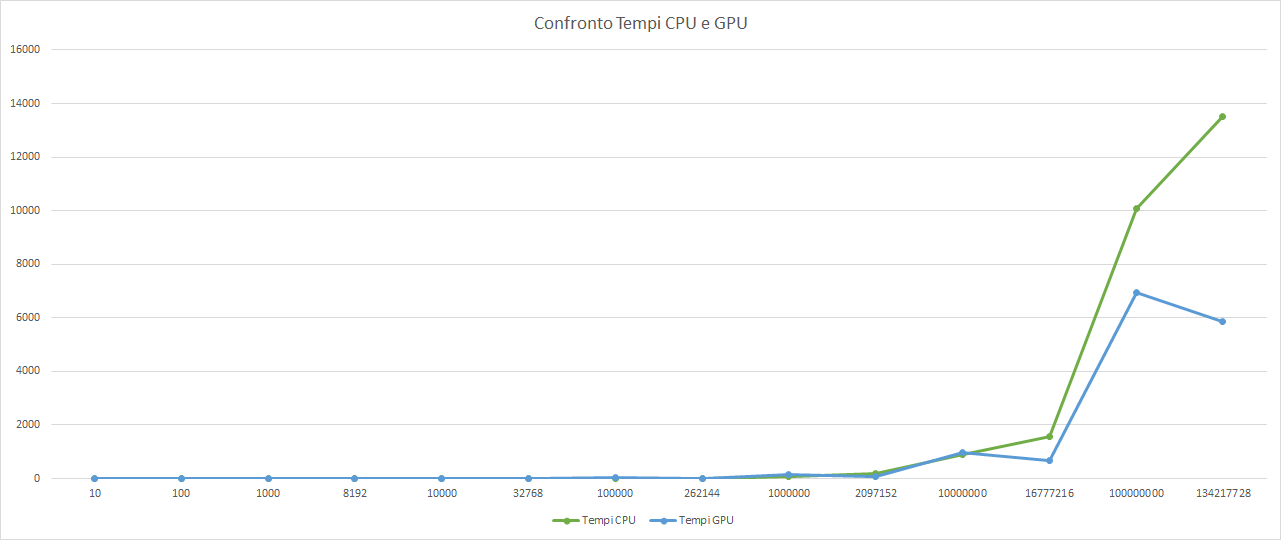
\includegraphics[width=0.99\linewidth]{img/ConfrontoTempi}
			\caption{Confronto tempi tra GPU e CPU}
			\label{fig:confrontotempi}
		\end{figure}
		
		Durante la fase di test è stata usata l'opzione -t con l'opzione -p 1234 (che setta il seme del generatore random) 
		per generare lo stesso array randomico da far ordinare sia al warpsort che al quicksort.
		
		Durante la fase di test è stata usata anche l'opzione -g, che permette di controllare che l'array ordinato sia effettivamente ordinato
		e contenga tutti e soli gli elementi dell'array di partenza. I test sono sempre stati passati.
		
		L'algoritmo consuma molta memoria GPU: ci sono due copie dell'array da ordinare e di sample 
		(infatti i kernel bitonic\_merge e bitonic\_merge\_2 usati nelle fasi 0, 2 e 4 hanno bisogno di due array distinti per input e output)
		oltre alla matrice local\_count.
		La memoria dedicata del mio PC è di soli 2GB e quindi non mi è stato possibile fare prove ulteriori 
		con array più grandi di $2^{27}$ elementi.
		
		Si può notare come la GPU, stranamente, sia più performante nel ordinare array senza padding.
		
		Nel confronto tra CPU e GPU si può notare come, per array di piccole dimensioni, la CPU sia notevolmente più veloce (fino all'ordine del 
		milione). Dai 10 milioni in su invece la GPU ha superato la CPU nelle performance. Purtroppo, come detto in precedenza, non è stato 
		possibile fare 
		test con array più grandi, ma verosimilmente il divario che si è creato dai 10 milioni è destinato ad aumentare col crescere 
		della dimensione dell'array.
	\section{Possibili sviluppi}
		L'uso di più di una GPU non è stato considerato perché durante lo sviluppo si è avuto accesso ad una sola GPU, ma non è difficile
		adattare l'algoritmo per poter sfruttare più GPU contemporaneamente. 
		In questo caso si prevede uno speedup delle prestazioni generali.
	\section{Sorgenti}
		\label{sorgenti}
		I sorgenti sono consultabili al seguente link: \url{https://github.com/Tovy97/WarpSort}
		
	\newpage
	\printbibliography		
\end{document}